% ====================================================================
% [挿入箇所例: 14.10 節末尾 または 14.10.1 節の直前/直後]
% ====================================================================

\chapter{実装：Flipper Zero による生体暗号解読のオフロード}
\begin{center}
    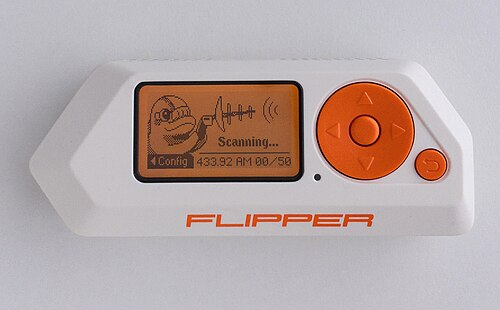
\includegraphics[width=0.7\linewidth,height=8cm,keepaspectratio]{./src/images/Flipper_Zero.jpg}
    \caption{Flipper Zero（Sub-GHzスキャンモード動作時）\newline
    {\tiny Photo by Jedi95 / Wikimedia Commons / CC BY-SA 4.0}}
    \label{fig:flipper_zero}
\end{center}
現場でのプロファイリングや対面観察において、プロファイラーの内部状態を
$\mathcal{S}(\mathrm{ZERO})$ に維持し、CEN（中央実行系）の計算リソースを相手の微小動作（$\lambda, \Lambda$）のキャリブレーションに $100\%$ 集中させるためには、デシバンの逐次暗算プロセスそのものを外部ハードウェアへとオフロードすることが極めて有効である。

この工学的要請に基づき、筆者が開発・公開しているオープンソース実装が、ポータブル生体観測インターフェース \textbf{Flipper Zero} 向けアプリケーションである。

本ツールは、観測事象 $D$ に対する $P(D \mid H)$ および $P(D \mid \neg H)$ の 4 段階スケール入力、チューリングの対数尤度比（deciban）のリアルタイム累積加算、判定閾値超過時の自律的通知（振動・音声・LED）、そして単一ステップの取り消し（Undo）機能を搭載している。これにより、観察者は自らの内部対話 $Ad$ を一切駆動させることなく、指先のブラインド操作のみで確信度 $\Omega$ の境界条件を物理的に追跡可能となる。

実装コード、UI操作マッピング、およびビルド手順の完全な仕様は、以下のオープンソース・リポジトリを参照されたい。

\begin{quote}
\small
\textbf{GitHub リポジトリ（ソースコードおよび仕様書）}:\\
\url{https://github.com/xsigil/flipperzero-othello-filter/blob/main/README.md}
\end{quote}

